\documentclass[a4paper]{article}

%% Language and font encodings
\usepackage[english]{babel}
\usepackage[utf8]{inputenc}
\usepackage{float}
\usepackage{booktabs}
\usepackage{tabu}
\usepackage{url}

%% Sets page size and margins
\usepackage[a4paper,top=2cm,bottom=2cm,left=2cm,right=2cm,marginparwidth=1.75cm]{geometry}

%% Useful packages
\usepackage{amsmath}
\usepackage{graphicx}
%\usepackage{apacite}
\usepackage[colorinlistoftodos]{todonotes}
\usepackage[colorlinks=true, allcolors=blue]{hyperref}

\title{LLM-Augmented Knowledge-Graph-Based Recommendation System
}
\author{Kartikey Chauhan - 501259284}
\date{}

\begin{document}
\maketitle
\section*{Overview}
Recommender systems have been widely applied to address the issue of information overload in various internet services, exhibiting promising performance in scenarios such as e-commerce platforms and media recommendations. 
In the general domain, the traditional knowledge recommendation method is  \textit{collaborative filtering (CF)}, which usually suffers from the cold start problem and sparsity of user-item interactions. 
Knowledge-based recommendation models effectively alleviate the data sparsity issue leveraging the side information in the knowledge graph, and have achieved state of the art performance\cite{guo2020survey} (e.g. KGAT\cite{wang2019kgat} , LightGCN\cite{he2020lightgcn}).
However, KGs are difficult to construct and evolve by nature, and existing methods often lack considering textual information. On the other hand, LLMs are black-box models, which often fall short of capturing and accessing factual knowledge.
Therefore, it is complementary to unify LLMs and KGs together and simultaneously leverage their advantages (See \hyperref[fig:llm_vs_kg]{Figure 1}).
This project aims to explore LLM-augmented KGs, that leverage Large Language models (LLM) for different KG tasks such as embedding, completion, construction and also incorporate textual information which could be a way to help overcome these challenges and lead to better recommendation systems.

\section*{Research Questions}

\begin{itemize}
\item Can LLM's be used to enhance the construction / quality / volume of information in the knowledge graphs? Is it possible to effectively constrain LLM output to be of a specific systematic knowledge extraction format?
\item Do these improved knowledge graphs lead to better recommendation systems? 
\item Can we combine current SOTA methods with the use of LLMs in extracting latent relationships, Knowledge Graph (KG) embedding, KG completion, and KG construction for recommendation in an efficient, explicit, and end-to-end manner.
\end{itemize}

\section*{Datasets}
\begin{itemize}
\item The primary dataset in scope is \href{https://amazon-reviews-2023.github.io/index.html}{Amazon Reviews'23}. If needed, the proposed system will also be extensively compared against baselines of state of the art models on popular recommendation datasets (e.g Amazon-book, Last-FM, Yelp2018). 
\end{itemize}
\section*{Evaluation}
\begin{itemize}
\item \textbf{AUC}, \textbf{Recall@K} and \textbf{Normalized Discounted Cumulative Gain (NDCG)} are chosen as key metrics to evaluate the performance of the proposed system. 
These metrics will provide a comprehensive assessment of the system's ability to accurately recommend items that are relevant to users. 
AUC measures the quality of the overall ranking of items, Recall@K evaluates the model's ability to recommend relevant items within the top K recommendations, and NDCG takes into account both the relevance and the rank of the recommended items.
\end{itemize}

\nocite{*}
\bibliographystyle{plain}
\bibliography{refs}

\section*{Appendix}

\begin{figure}[H]
\centering
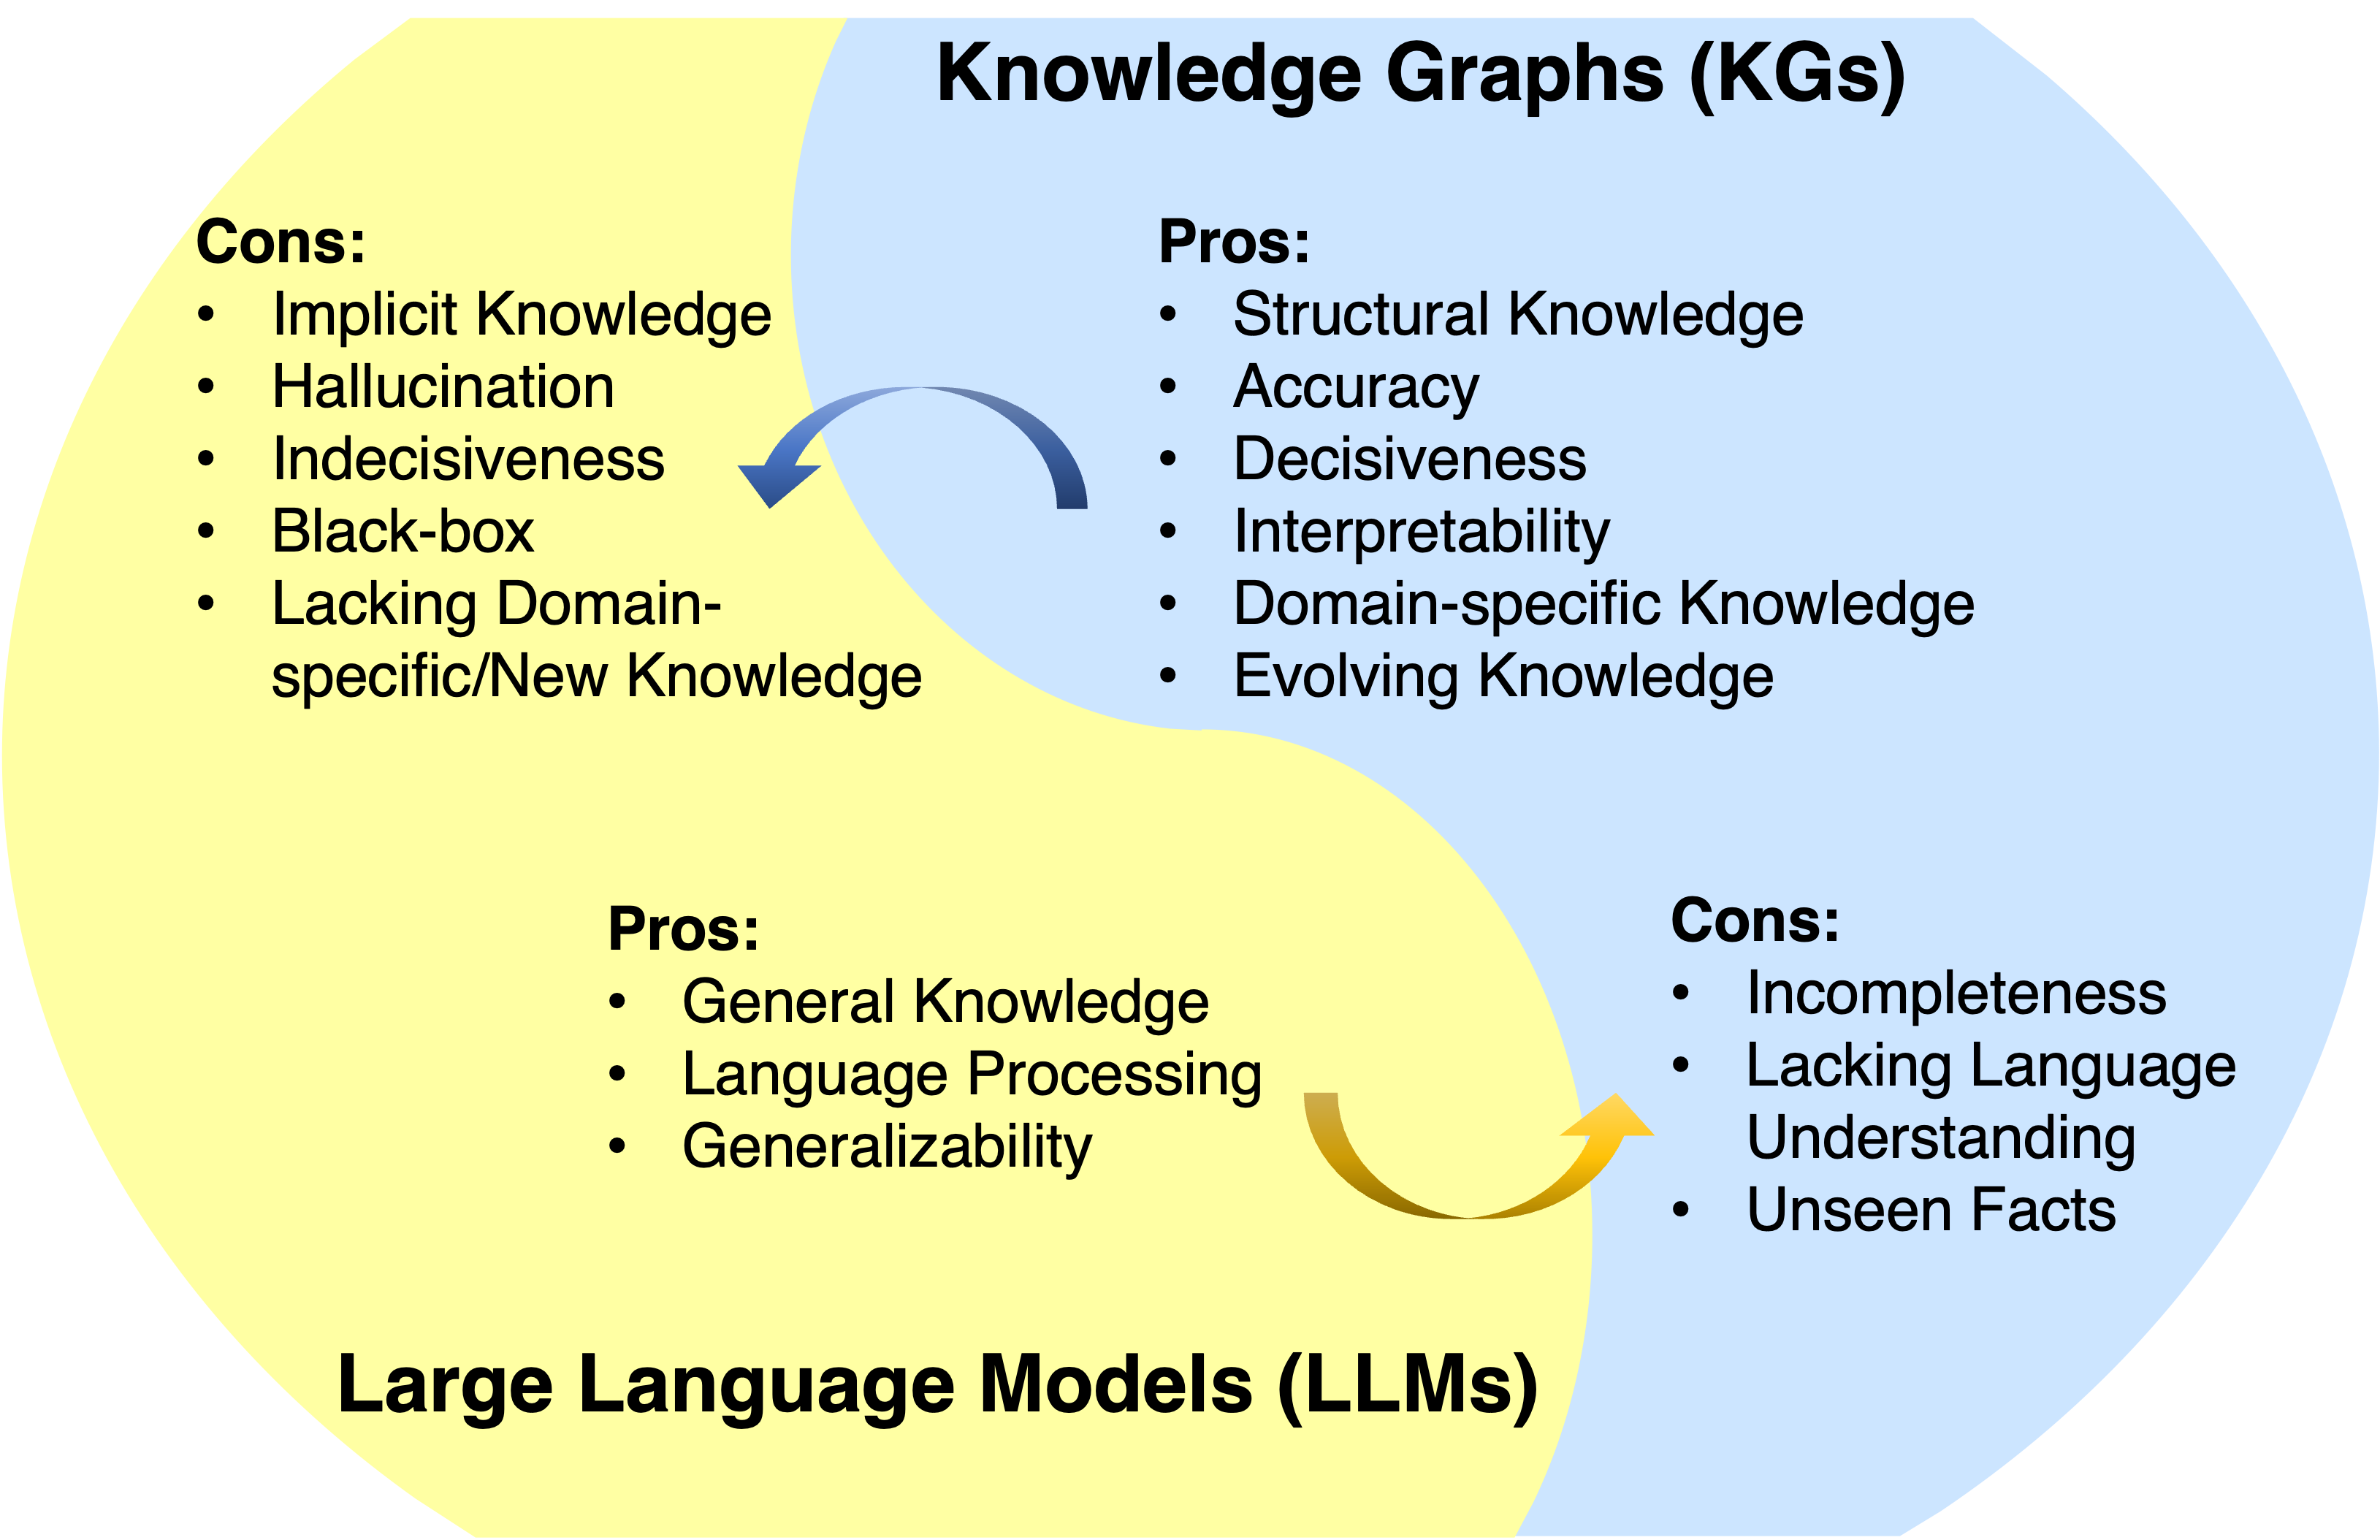
\includegraphics[width=0.6\textwidth]{img/PLM_vs_KG.png}
\caption{Summarization of the pros and cons for LLMs and KGs. From \cite{pan2023unifying}.}
\label{fig:llm_vs_kg}
\end{figure}


\begin{figure}[H]
\centering
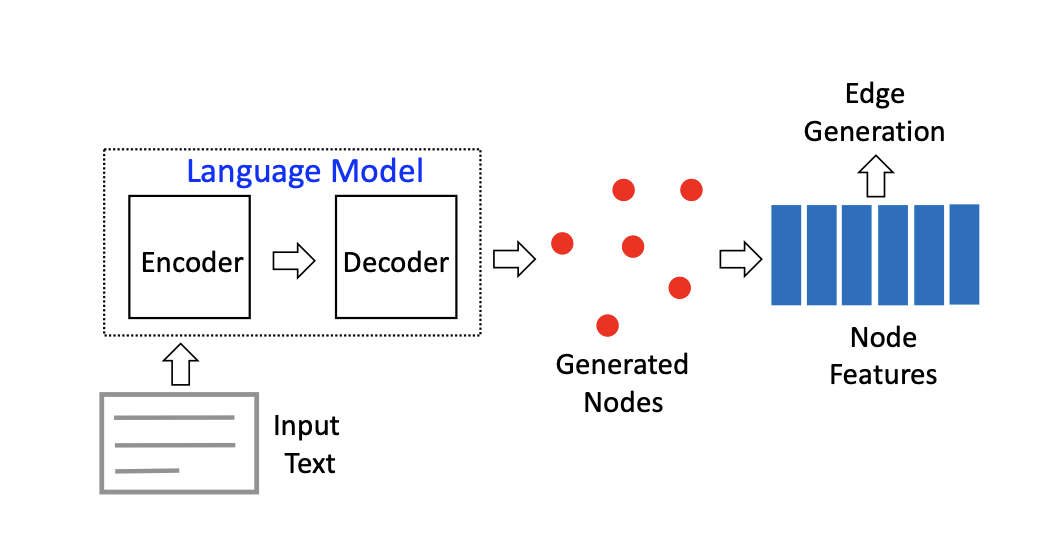
\includegraphics[width=0.8\textwidth]{img/Idea.png}
\caption{High level overview of constructing Knowledge Graphs from Language models.}
\label{fig:kg_construction}
\end{figure}
    
\begin{figure}[H]
\centering
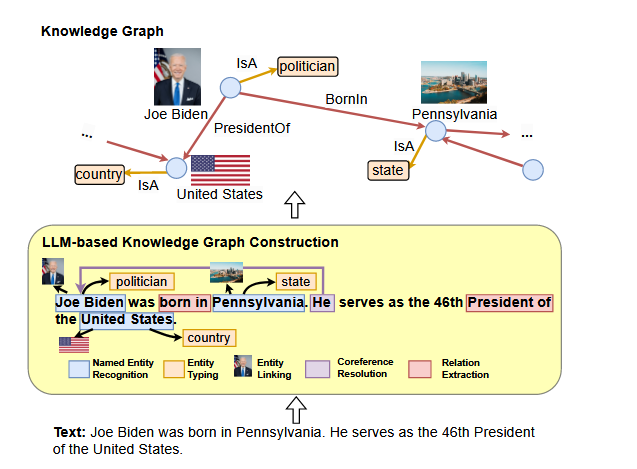
\includegraphics[width=0.8\textwidth]{img/KG_construction.png}
\caption{The general framework of LLM-based KG construction. From \cite{pan2023unifying}.}
\label{fig:kg_construction}
\end{figure}

\begin{figure}[H]
\centering
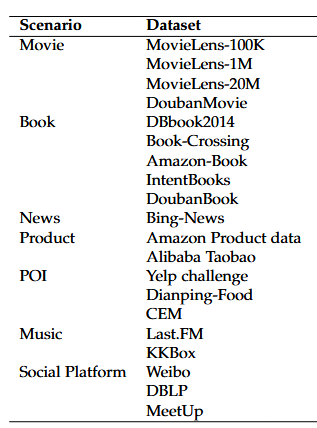
\includegraphics[width=0.3\textwidth]{img/datasets.png}
\caption{A collection of datasets for different application scenarios. From \cite{guo2020survey} }
\label{fig:datasets}
\end{figure}

\end{document}